\documentclass[10pt,a4paper,twocolumn]{article}

\input{pisika.dat}

%  Editorial staff will uncomment the next line
% \input{staff.hed}


\begin{document}

%--------------------------------------------------------------------------
%  fill in the paper's title, author(s), and corresponding institutions
%--------------------------------------------------------------------------
\providecommand{\ShortAuthorList}[0]{A.~M.~Surname, B.~D.~Suffix Jr., C.~G. Suffix III} % use "A.~M.~Surname \textit{et al}." for more than three authors.
\title{Modelování hledání potravy v mravenčí kolonii}
\author[1]{Autor David Beinhauer}
\affil[1]{Department of Physics, DD University}
\affil[2]{Department of Science, XX University}

\date{\dateline{}}

\begin{abstract}
\noindent
%---------------------------------------------------------------------------
%               Include abstract and keywords here
%---------------------------------------------------------------------------
Chování hmyzích druhů žijících v kooperujících koloniích je dodnes 
výzvou pro vědu. Pochopení této problematiky může vést k zdokonalení řešení
řady zdánlivě nesouvisejících problémů. V práci je představen jednoduchý
multiagentní model mravenčí kolonie zaměřující se na problematiku shánění
potravy v různě komplexních prostředích. Návrh modelu je inspirován prací 
\citet{jones2010characteristics}. 
Při analýze (TODO: dopsat vysledky analyzy)

\keywords{keyword 1, keyword 2}

\DOI{} % do not delete this line
\end{abstract}

\maketitle
\thispagestyle{titlestyle}



%---------------------------------------------------------------------------
%               the main text of your paper begins here
%---------------------------------------------------------------------------
\section*{Úvod}

Kolektivní chování řady druhů hmyzu, mezi než patří například mravenci,
je charakteristické komplexností a vysokou koordinovaností jedinců. Kolonie
mravenců například společně zajišťuje potravu pro celou populaci, buduje hnízdo,
strará se o potomky, či se brání před predátory. Pochopení tohoto chování by
mohlo pomoci zdokonalit řešení řady zdánlivě vzdálených problému, mezi něž
patří například problém obchodního cestujícího (TODO: reference) a řada dalších. 
jedinců, komplexnosti přirozeného prostředí a nepřesnosti měřících zařízeních 
je však exaktní studium chování a organizace těchto kolonií velmi komplikované a 
často značně nepřesné. V důsledku nárustu výpočetního výkonu se v současnosti 
pro studium takto komplexních dějů stále častěji využívají matematické modely. 

V této práci navrhujeme a analyzujeme jednoduchý multiagentní model mravenčí 
kolonie zaměřený na problematiku shánění potravy. Model je založen na komunikaci
mravenců pomocí vypouštění a detekce rozdílné hladiny feromonů v prostředí.
Z velké části je insporován prací \citet{jones2010characteristics}, jenž studuje
formování transportních drah plísně \emph{Physarum polycephalum}. V analytické části
porovnáváme chování mravenců a jejich úspěšnost při sběru potravy v různě 
strukturovaných prostředích. Dále zkoumáme závislosti počtu jedinců a jejich 
schopnosti dopředu detekovat cílovou destinaci na celkovém množství potravy 
dopravené do hnízda v průběhu simulace. 


\section*{Matematický model}
Při návrhu modelu jsme se zaměřili především na jednoduchou architekturu s
malým množstvím snadno pochopitelných parametrů pro jednodušší analýzu 
fungování modelu, který vhodně popíše chování mravenců při hledání potravy.
Ideálně by měl model zachytit kolektivní chování mravenců při hledání potravy.
Mravenci by měli být schopni jednoduchou lokální signalizací pomocí
vypouštění feromonu co nejvíce optimalizovat trasu pro zásobování hnízda
potravou. V modelu je dále možné zkoumat různé varianty map s různě 
rozmístěnými překážkami, hnízdy i potravou.

\section*{Výsledky}

V analýze modelu jsme se zaměřili především na chování mravenců v různých
variantách prostředí. Dále jsme se zaměřili na závislost počtu
jedinců (parametr $n$) a maximální vzdálenosti pro detekci hledaného 
objektu (parametr $d$). Zbylé parametry jsme zvolili pevně na základě
porovnávání výsledků pro různé hodnoty. 

\subsection*{Varianty map}
Pro analýzu modelu jsme zvolili celkem 6 variant mapy s účelem otestovat
chování modelu v prostředích s odlišnou charakteristikou. Zvolili jsme 
jednotnou velikost mřížky prostředí, jež je rovna $100 \times 100$.
Jednotlivé varianty se liší rozmístěním zdrojů potravy, mraveniště a překážek
v prostředí.

Základní varianta prostředí (ozn. jako \texttt{var-0}), jež je použita 
také pro výběr parametrů, neobsahuje žádnou překážku. Prostředí obsahuje 
jediné mraveniště umístěné přibližně uprostřed mapy a dva zdroje potravy
umístěné v rozích mapy na společné diagonále. Zdroje potravy se od sebe 
mírně liší vzdáleností od hnízda a velikostí. Další varianta 
(ozn. \texttt{var-1}) je téměř identická vůči variantě
\texttt{var-0}. Liší se však v obklopení téměř celého zdroje
potravy překážkami s pouze malým prostorem pro vstup mravenců. Následující
varianta (ozn. \texttt{var-2}) je jednoduché symetrické bludiště s hnízdem 
na levém konci. Okolí hnízda je ohraničeno překážkami, jež vytváří podélný 
průchod pro mravence směrem k potravě. V pravé části mapy je umístěno 
rozdvojením na jejichž koncích jsou zdroje potravy. Úsek od rozdvojení
k potravě je kratší než od hnízda k rozdvojení. Velmi podobné je rozložení
další varianty (\texttt{var-3}). Lišící se od \texttt{var-2} pouze ve 
vzdálenostech hnízda od rozdvojení, která je kratší, a rozdvojení od 
zdrojů potravy, které jsou delší. Další z variant (ozn. jako \texttt{var-5})
je v rozložení téměř totožná jako \texttt{var-2}. Liší se pouze v tom, že 
jedna větev bludiště neobsahuje zdroj potravy. Poslední varianta (ozn. jako
\texttt{var-4}) je koncipována jako průchod ve středu mapy s konci 
obsahujícími zdroje potravy. Hnízdo je umístěno ve středu mapy, je 
podélně ohraničeno překážkami vytvářející průchod. Na levém a pravém konci
mapy jsou umístěny zdroje potravy. Obrázek (\ref{fig:map_variants})
nabízí grafické znázornění rozložení variant prostředí.
 

\begin{figure}[tb]
  \centering
  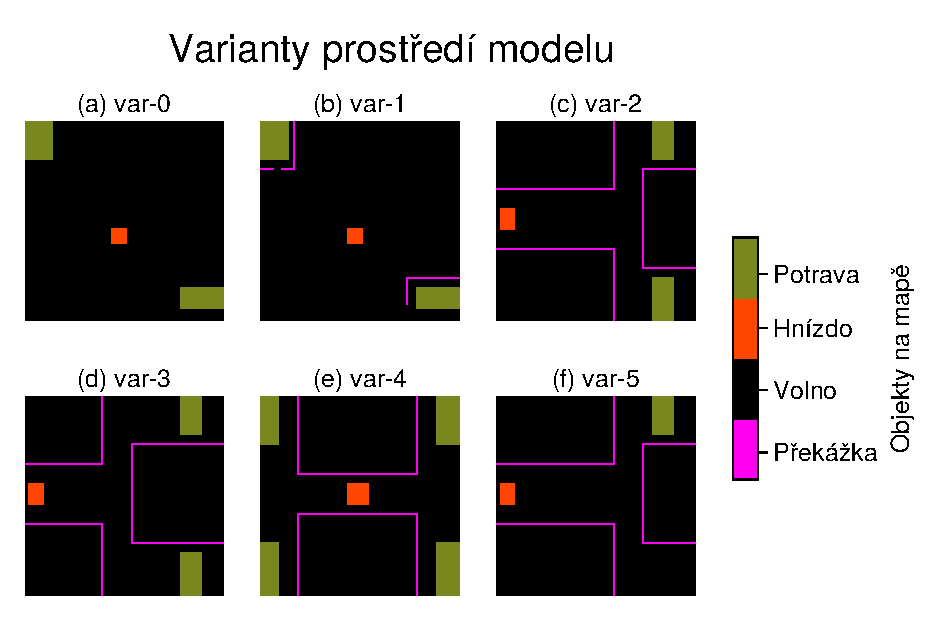
\includegraphics[width=0.9\linewidth]{images/maze_variants.pdf}
  \caption{Zobrazení variant prostředí modelu použité v experimentech. 
  Barevně rozlišujeme objekty v prostředí. Zeleně jsou označeny
  bloky potravy, červeně hnízda, fialově překážky na mapě, černě 
  je označena volná pozice bez speciálního objektu. Poznamenejme, že
  varianty \texttt{var-2}, \texttt{var-3}, \texttt{var-4}
  a \texttt{var-5} jsou koncipovány jako labyrinty a cíleně je zde část
  mapy nedosažitelná (ohraničená překážkami).}
  \label{fig:map_variants}
\end{figure} 

\subsection*{Porovnání variant prostředí}

Během experimentů jsme porovnávali především úspěšnost sesbírání potravy 
mravenci v různých variantách prostředí s různým počtem mravenců a různou
vzdáleností detekce hledaného objektu. 


% TODO: vsechny labely obrazku nize

\begin{figure}[tb]
  \centering
  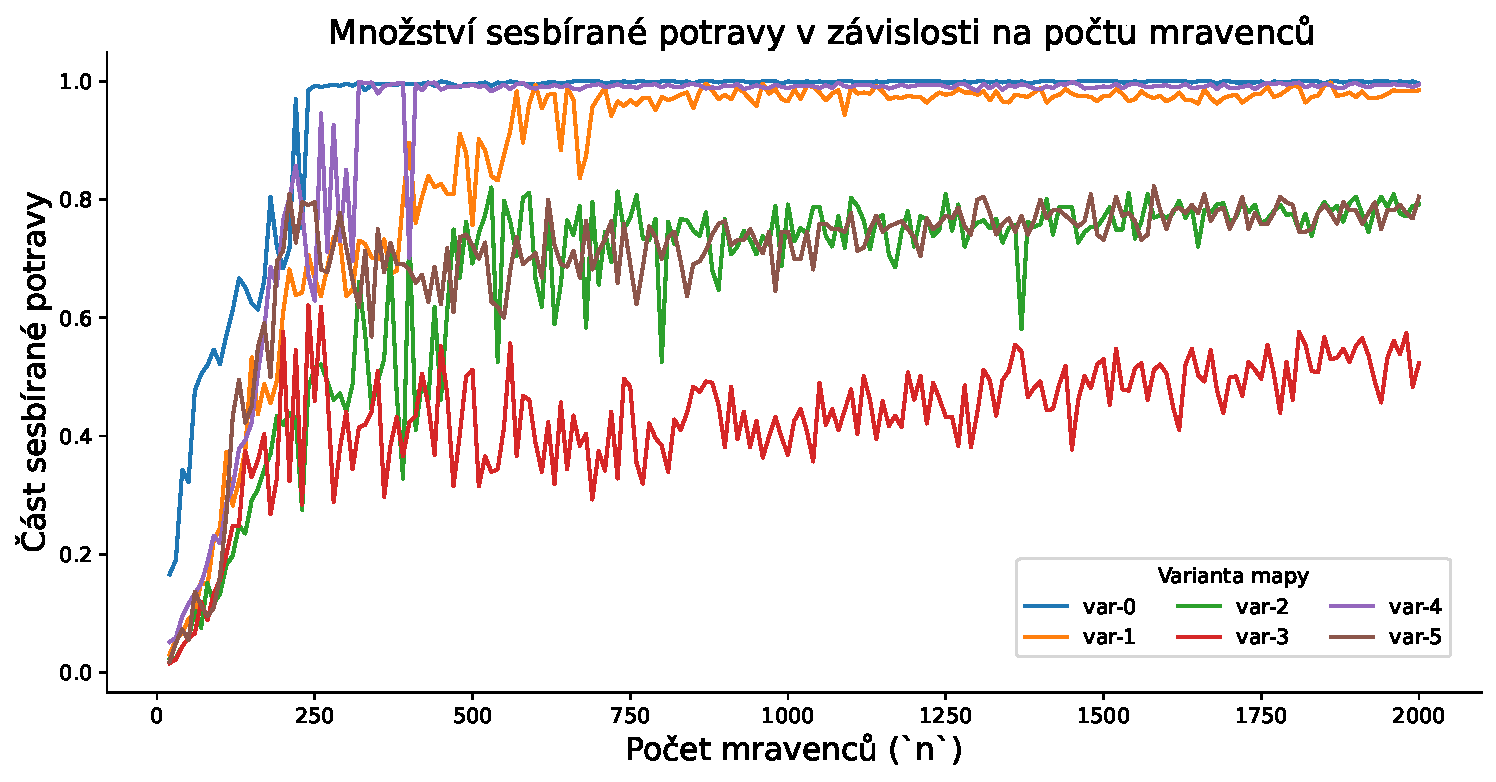
\includegraphics[width=0.98\linewidth]{images/num_ants_variants_together.pdf}
  \caption{}
  \label{fig:num_ants_together}
\end{figure}

\begin{figure}[tb]
  \centering
  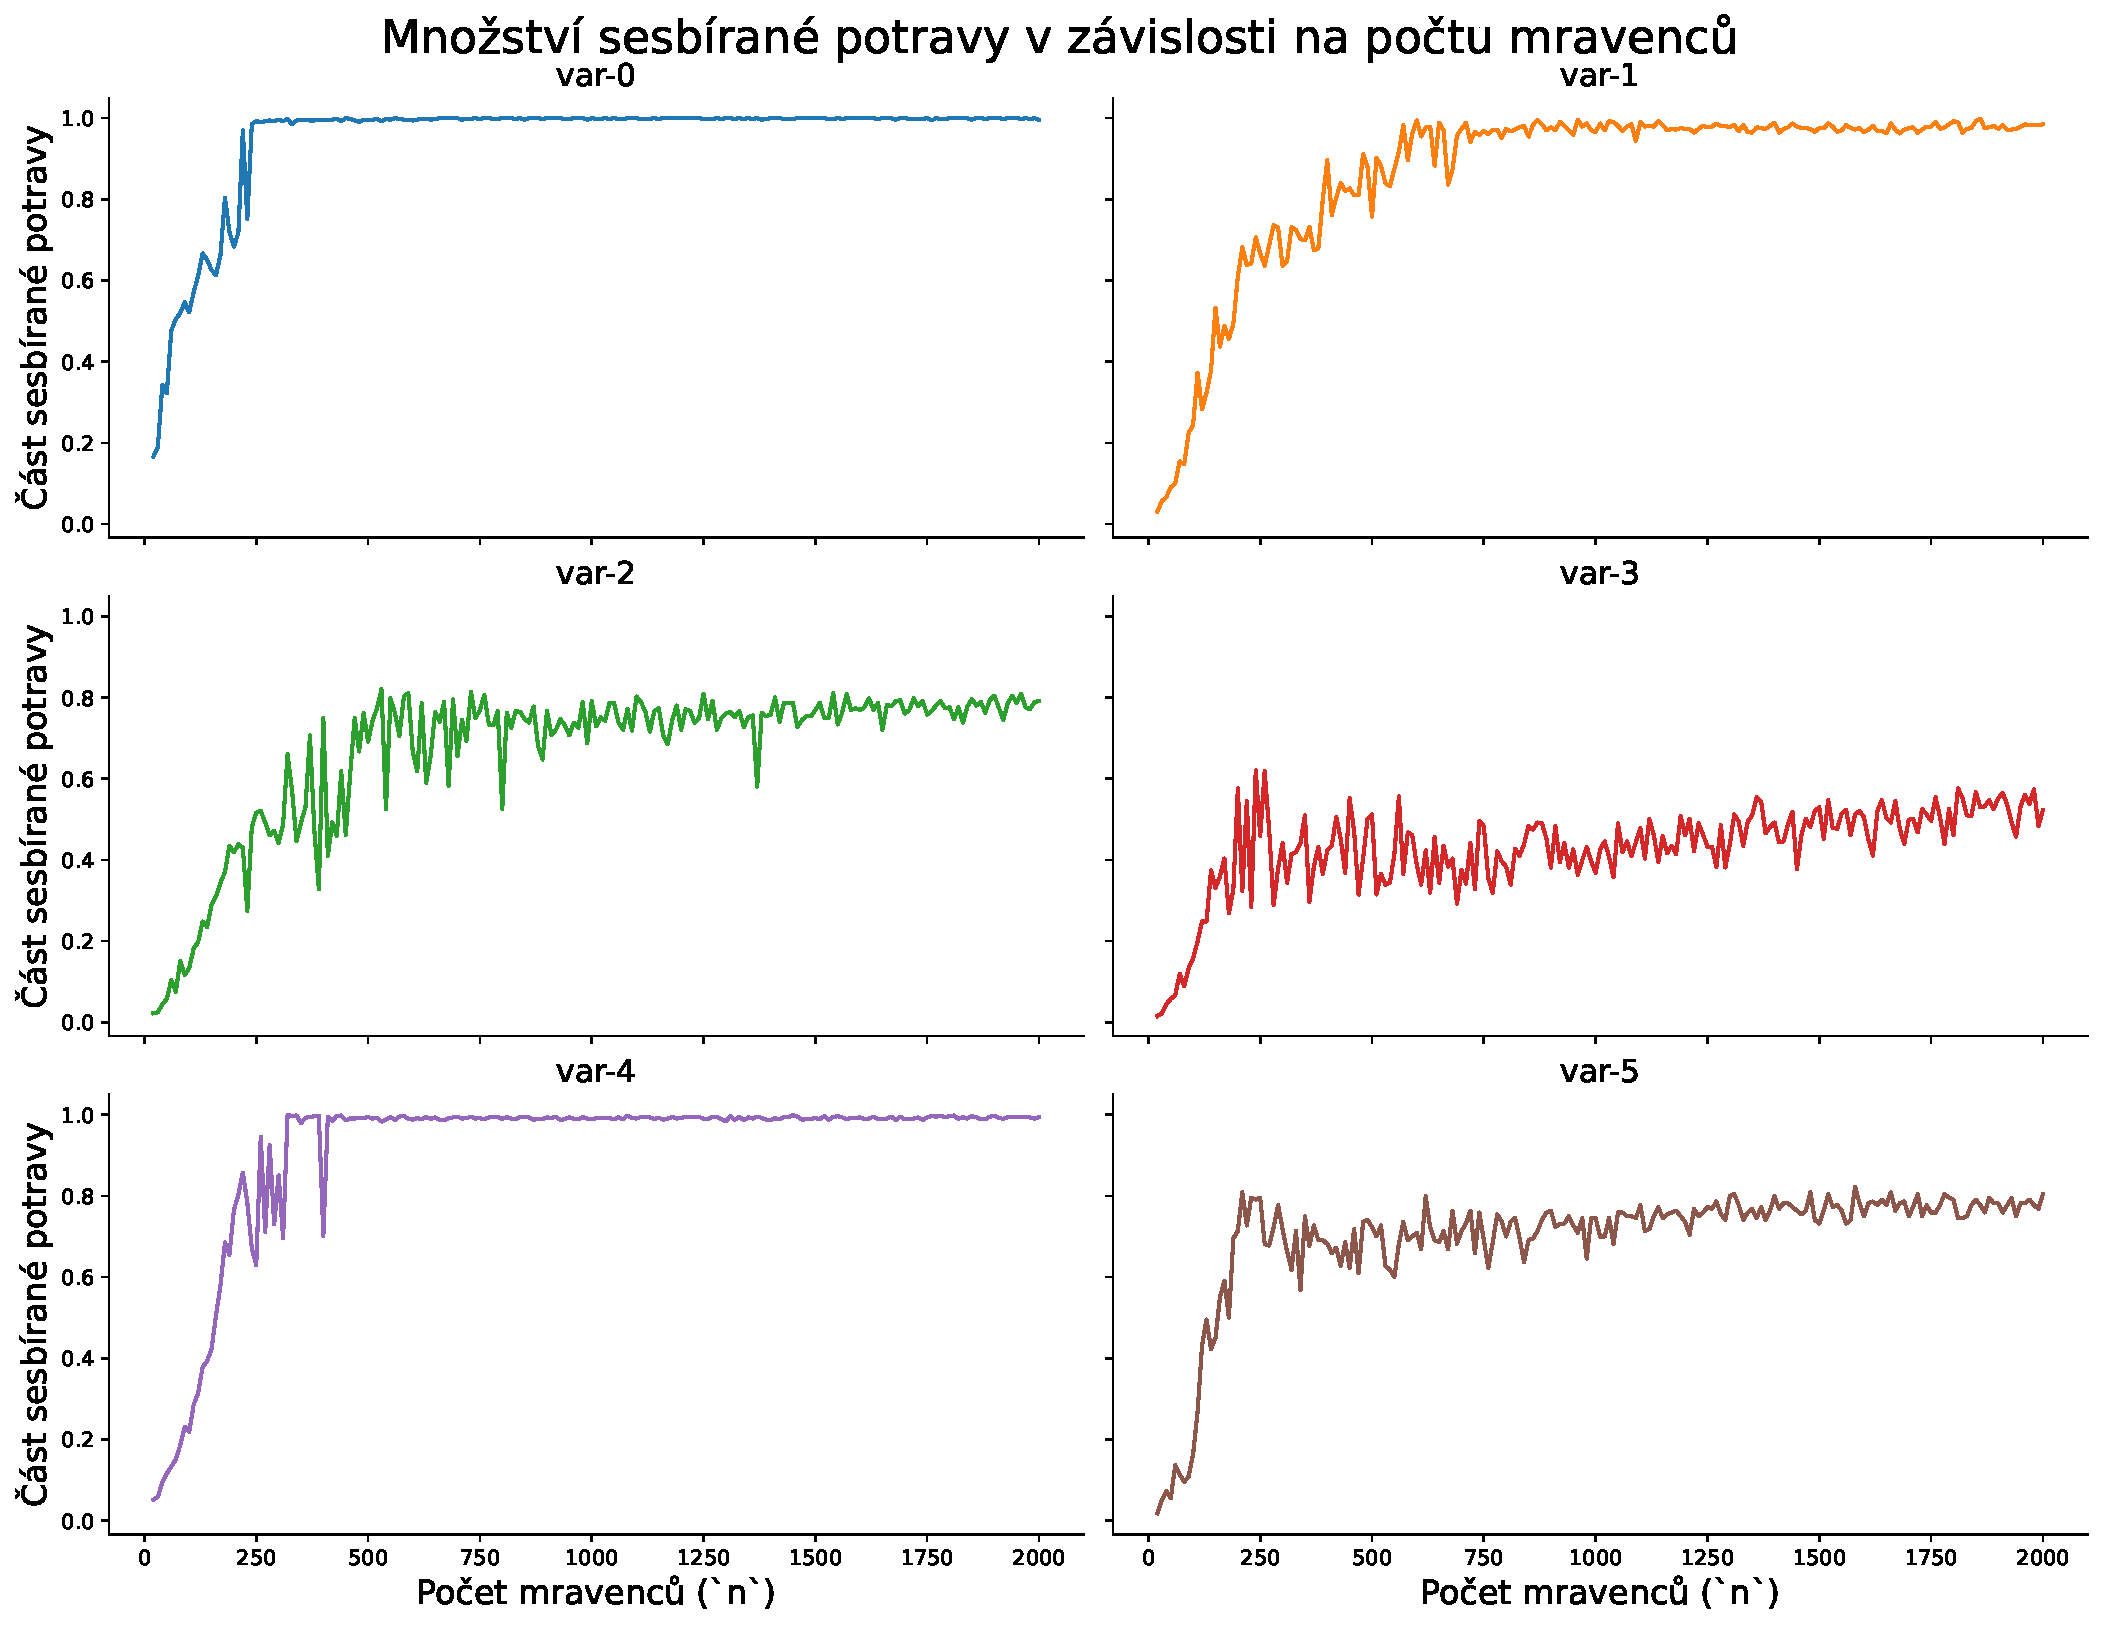
\includegraphics[width=0.98\linewidth]{images/num_ants_variants_separated.pdf}
  \caption{}
  \label{fig:num_ants_separated}
\end{figure}

\begin{figure}[tb]
  \centering
  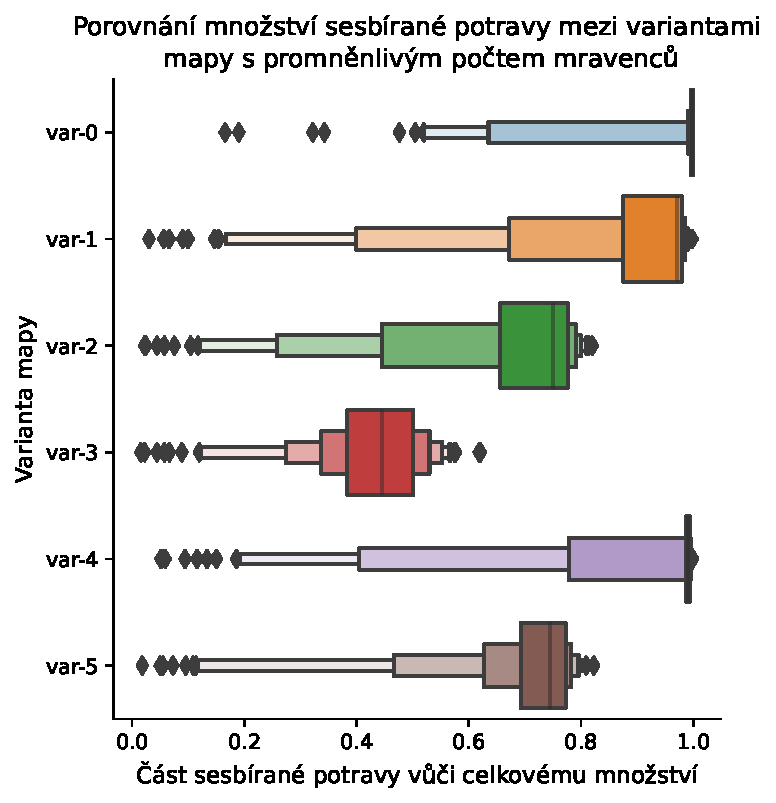
\includegraphics[width=0.98\linewidth]{images/num_ants_variants_means.pdf}
  \caption{}
  \label{fig:num_ants_means}
\end{figure}

\begin{figure}[tb]
  \centering
  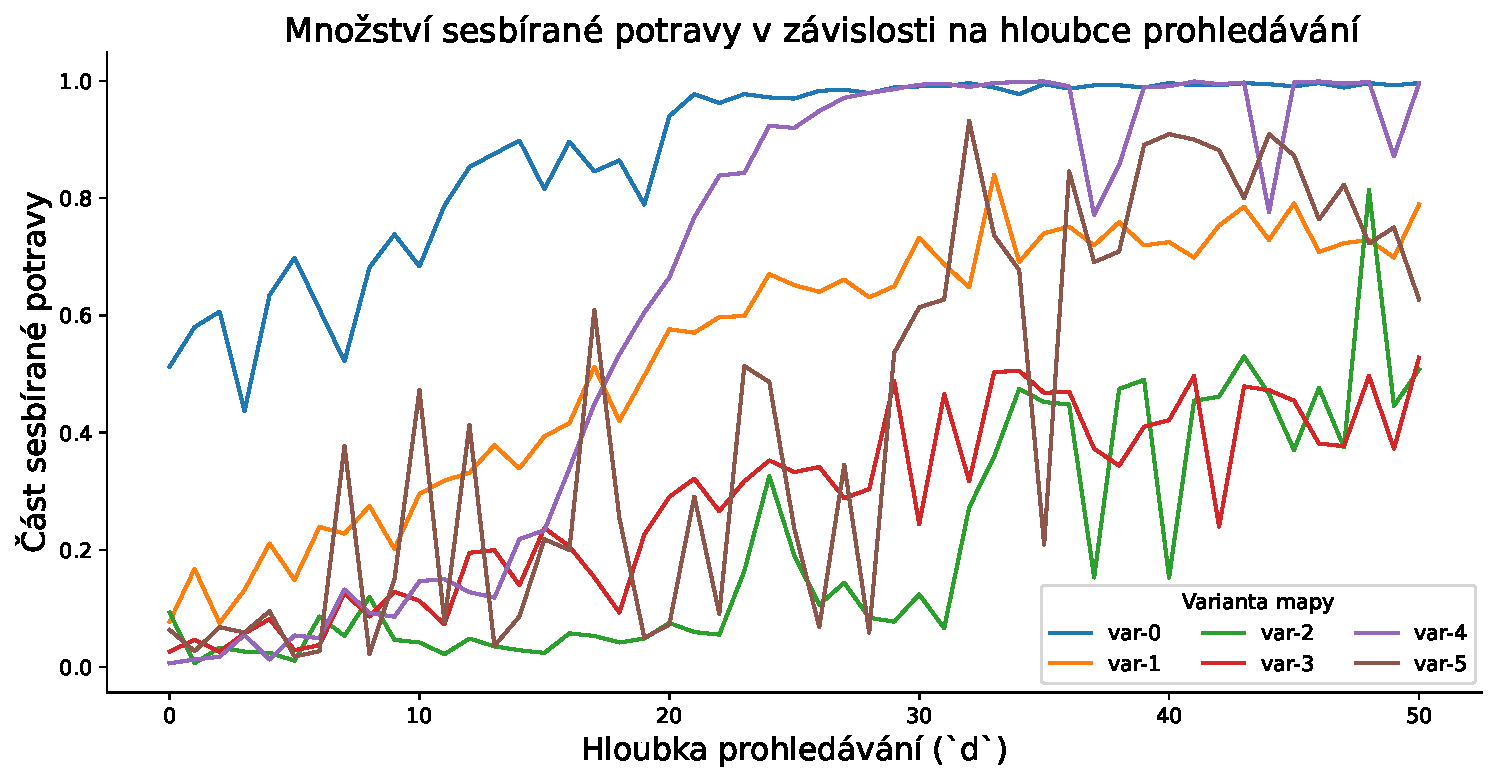
\includegraphics[width=0.98\linewidth]{images/search_depth_variants_together.pdf}
  \caption{}
  \label{fig:search_depth_together}
\end{figure}

\begin{figure}[tb]
  \centering
  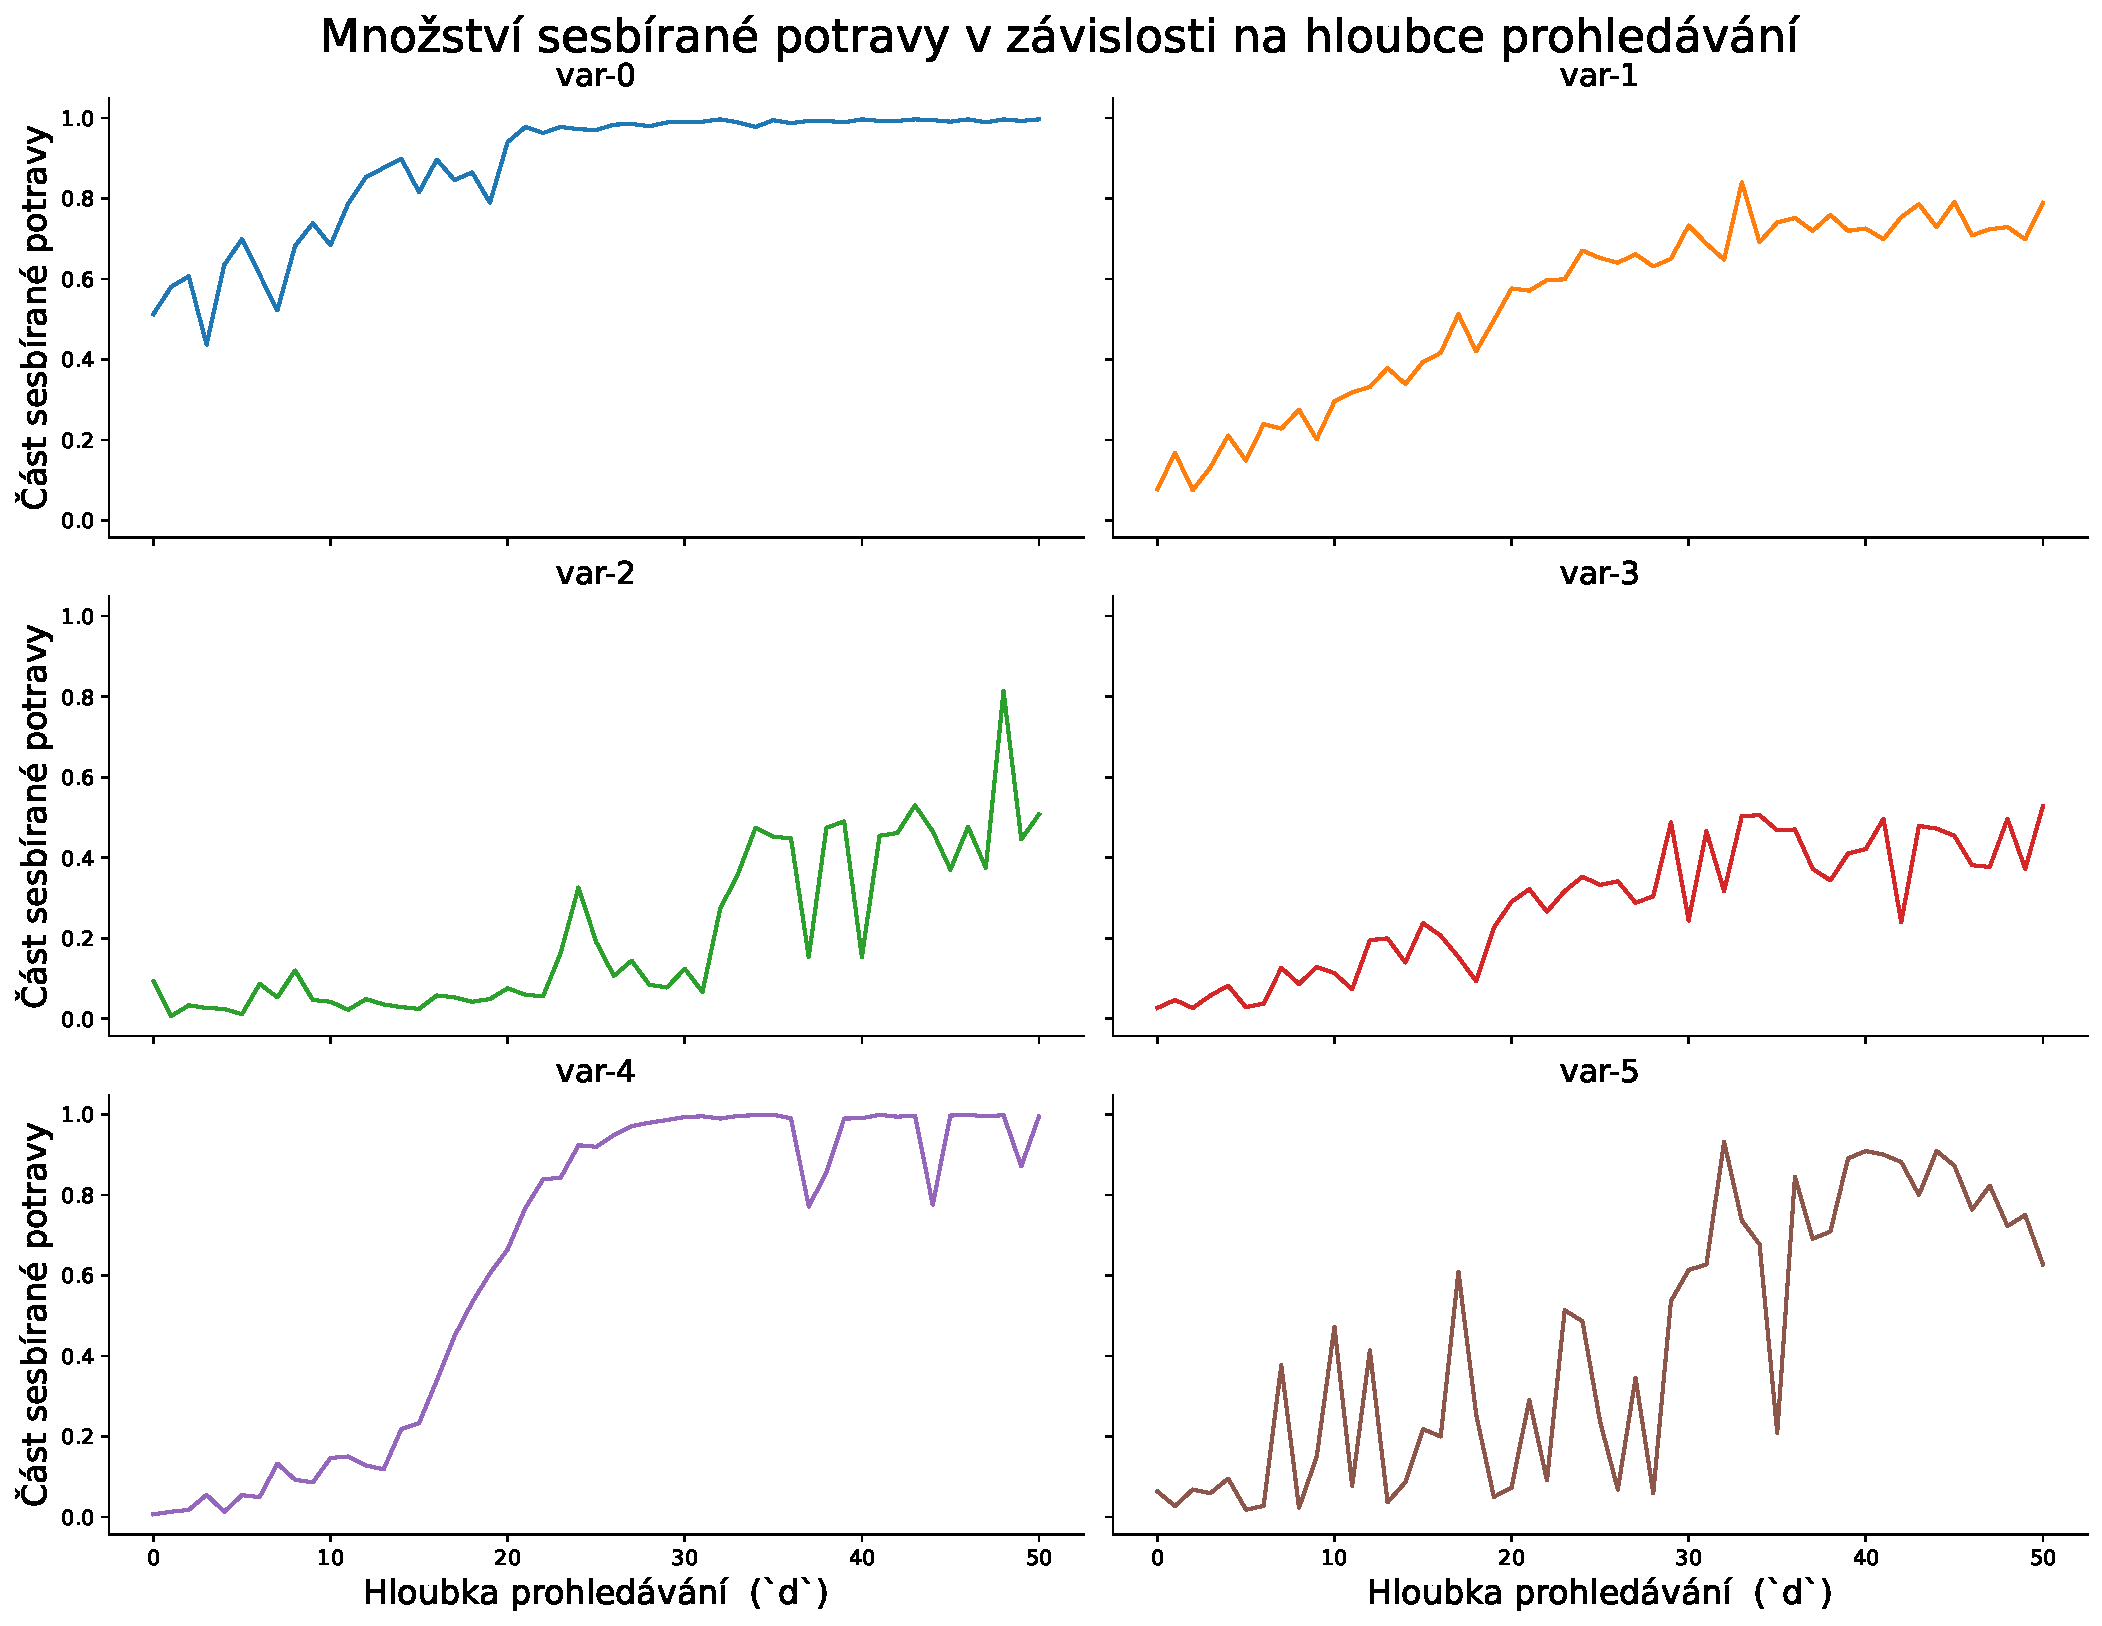
\includegraphics[width=0.98\linewidth]{images/search_depth_variants_separated.pdf}
  \caption{}
  \label{fig:search_depth_separated}
\end{figure}

\begin{figure}[tb]
  \centering
  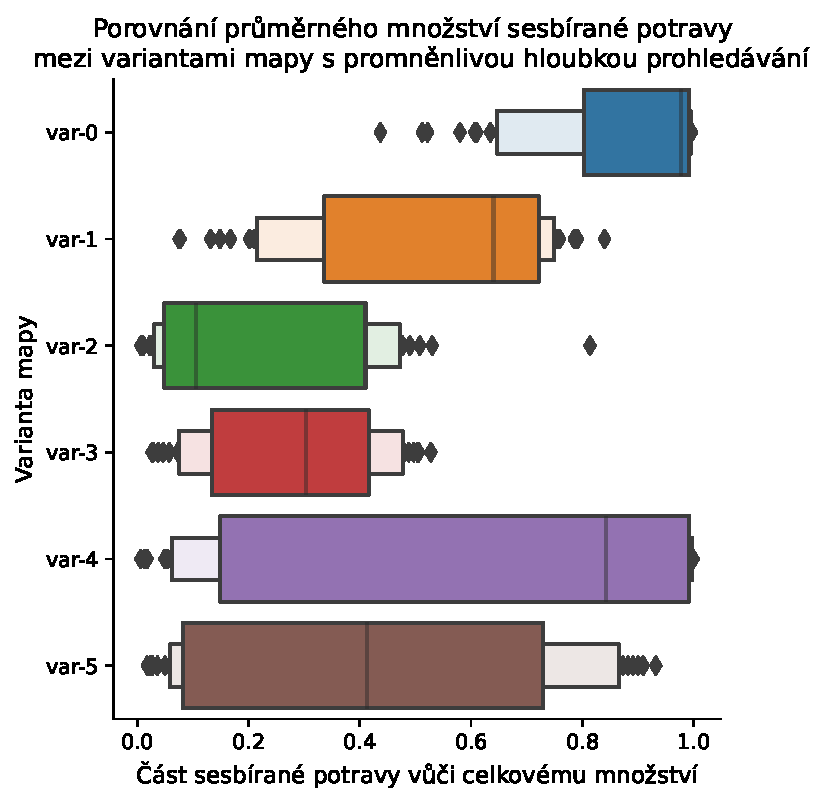
\includegraphics[width=0.98\linewidth]{images/search_depth_variants_means.pdf}
  \caption{}
  \label{fig:search_depth_means}
\end{figure}



\begin{figure}[tb]
  \centering
  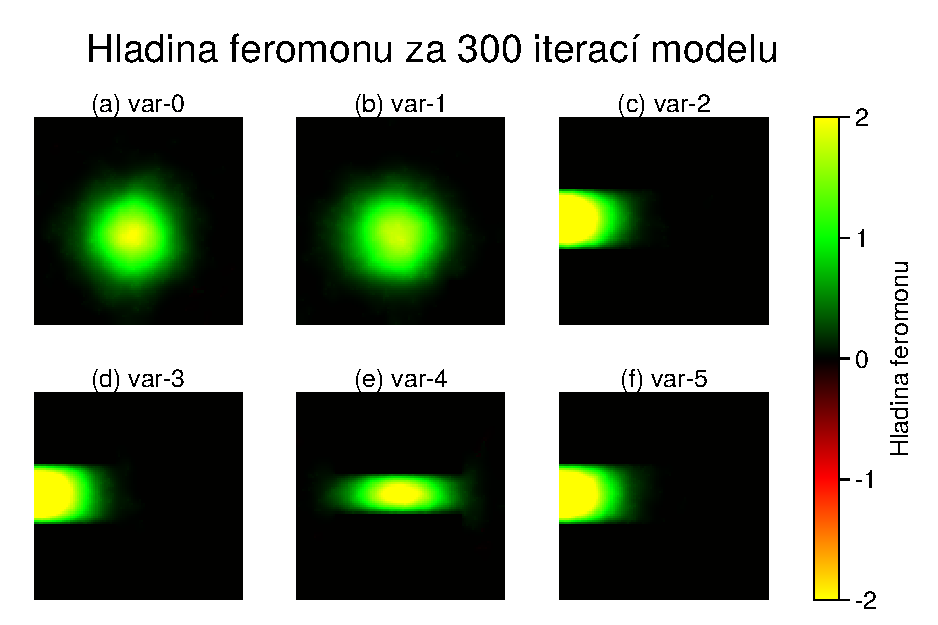
\includegraphics[width=0.9\linewidth]{images/pheromone_levels_300.pdf}
  \caption{}
  \label{fig:pheromones_300}
\end{figure}

\begin{figure}[tb]
  \centering
  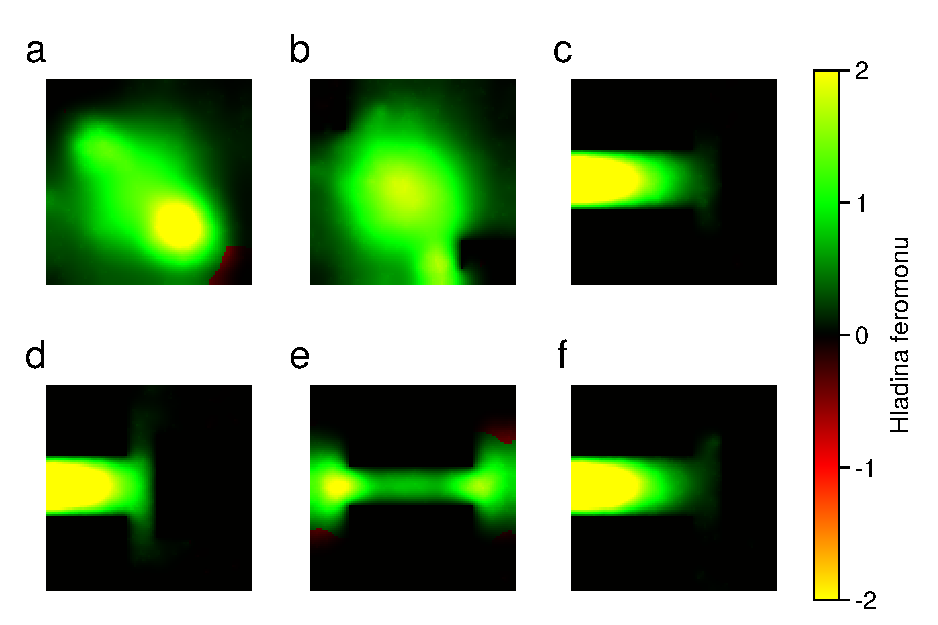
\includegraphics[width=0.9\linewidth]{images/pheromone_levels_1000.pdf}
  \caption{}
  \label{fig:pheromones_1000}
\end{figure}

\begin{figure}[tb]
  \centering
  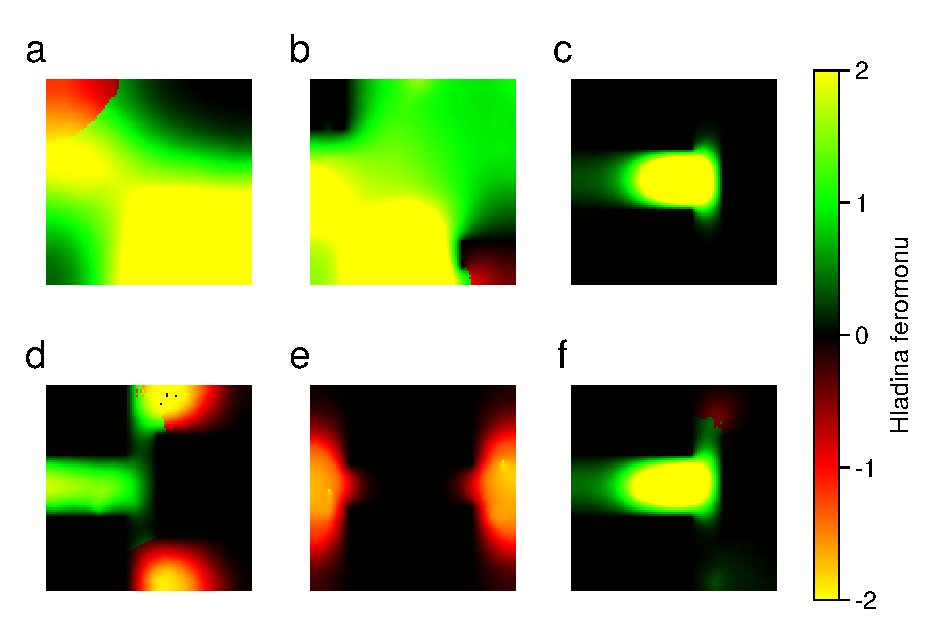
\includegraphics[width=0.9\linewidth]{images/pheromone_levels_4000.pdf}
  \caption{}
  \label{fig:pheromones_4000}
\end{figure}




TODO: porovnat jednotlive mapy

TODO: popsat zavislost poctu mravencu a hloubky prohledavani na poctu potravy



\section*{Metody}

\subsection*{Návrh modelu}
Model staví na návrhu z práce \citet{jones2010characteristics}
modelující formování transportních drah plísně \emph{Physarum polycephalum}
pomocí chemotaxe. Tento model jsme zvolili, jelikož je založen na podobných 
principech jako námi zkoumaný problém.

Použili jsme multiagentní model v diskrétním prostředí. Prostředí reprezentujeme 
pravidelnou 2D mřížkou, v níž každá buňka odpovídá pozici v simulovaném prostředí a je 
popsána množinou odpovídajících proměnných popsaných v tabulce (\ref{table:mapa}).
V prostředí jsou vždy omezené zásobárny potravy, kde každá buňka s potravou
odpovídá množství zásob, které je schopen přepravit jeden mravenec. Pokud
tedy mraven sebere potravu z dané buňky, pak se veškeré zásoby potravy v 
buňce vyčerpají a stane se tak prázdnou. Naopak předpokládáme, že všechny
buňky náležící hnízdu mají neomezenou kapacitu a je v nich možné 
nashromáždit neomezené množství potravy.


\begin{table}[t]
  \centering % center-align tables within a column
  \begin{tabular}{l p{5cm}}
  \toprule
  Proměnná & Popis \\
  \midrule
    \texttt{map\_object} & Objekt v buňce (možnosti:
    žádný, překážka, potrava, mraveniště). \\
    \texttt{food\_pheromone} & Hladina feromonu pro sběr potravy.\\
    \texttt{nest\_pheromone} & Hladina feromonu pro návrat do mraveniště.\\	
  \bottomrule
  \end{tabular}
  \caption{Seznam promměnných jedné buňky mapy simulace.} \label{table:mapa} 
\end{table}


Agenti reprezentují jednotlivé mravence a jsou náhodně 
vygenerování v mraveništích začátku simulace. Jejich počet je dán 
parametrem \texttt{num\_ants} a 
v průběhu simulace je již neměnný. Jsou charakterizováni pozicí na mapě,
orientací a příznakem, zda hledají potravu, nebo se s ní vracejí do mraveniště.
Každý agent v každém kroku simulace provede následující posloupnost akcí:

\begin{enumerate}
  \item Podle svého stavu zkontroluje, zda se nachází u zdroje potravy 
  (resp. v mraveništi). Pokud ano, pak sebere jednotku potravy 
  (resp. vyloží ji v mraveništi) a náležitě změní stav.
  \item Přesune se na novou pozici.
  \item Vypustí jednotku odpovídajícího feromonu na nové pozici.
\end{enumerate}

Mravenec má v každém kroku simulace pouze 3 možné varianty posunu, které 
jsou posun o 1 pozici vpřed, doleva nebo doprava. Z výběru jsou následně vyřazeny
pozice s překážkami a vyskytující se mimo mapu. Jestliže není ani jeden ze zmíněných 
pohybů možný, pak agent uniformě náhodně změní svou orientaci doleva, nebo
doprava. V opačném případě je nová pozice náhodně zvolena z vážené distribuce, 
v níž je váha možné nové pozice $p$ agenta $a$ rovna:

\begin{equation}
  weight(p, a) = pheromone(p, a) + c
\end{equation}

Kde $pheromone$ je funkce, jejíž hodnota je rovna hladině odpovídajícího 
feromonu na pozici $p$. Pokud mravenec hledá potravu, pak sleduje hladiny \texttt{food}
feromonu, v opačném případě \texttt{nest} feromonu.
Parametr $c$ slouží jako faktor pro snížení vlivu hladiny feromonu na volbě
nové pozice. Navíc pokud je mravenec dostatečně blízko cílovému objektu
v alespoň jednom z možných směrů (přímo, vlevo nebo v vpravo) a cesta
není blokována překážkou, pak se vždy posune směrem k tomuto objektu (viz.
parametr $d$ v tabulce (\ref{table:parametry})). 

Pro komunikaci mravenců používáme dvě varianty feromonů. Jeden pro označení 
cesty ke zdroji potravy, druhý pro signalizaci cesty do mraveniště. 
Každý mravenec v každé iteraci simulace vypustí aktuální pozici, buď feromon typu
\texttt{food}, pokud hledá potravu, nebo \texttt{nest}, pokud se s potravou
vrací do hnízda. Aby nedocházelo k hromadění feromonu, je koncentrace feromonu
na dané pozici shora omezena a v případě překročení hranice již nelze hladinu
feromonu dále zvyšovat. Vyprchávání feromonu v čase je realizováno následující 
diferenční rovnicí:

\begin{equation}
  level_{p}(t+1) = 
  \left\{
    \begin{array}{ll}
      level_{p}(t) - f  & level_{p}(t) > f \\
      0 & level_{p}(t) \leq f \\ 
    \end{array}
  \right.
\end{equation}

Kde $level_{p}(t)$ značí hladinu feromonu na pozici $p$ v čase $t$ a $f$
udává rychlost vyprchávání feromonu.

Dále je v každém kroku simulace část feromonu na libovolné pozici $p$ 
rovnoměrně difundována do Moorova okolí $p$ z nějž jsou vyřazeny neplatné pozice
(mimo mapu nebo překážky), množství difundovaného feromonu je dáno 
příslušným parametrem.

Tabulce (\ref{table:parametry}) obsahuje podrobnější popis parametrů modelu.


\begin{table}[t]
  \centering % center-align tables within a column
  \begin{tabular}{l p{5cm}}
  \toprule
  Parametr & Popis \\
  \midrule
    $n \in \mathbb{N}$ & Počet mravenců v simulaci 
    (\texttt{num\_ants}). \\ 
    $f \in (0, 1)$ & Rychlost vyprchávání feromonu 
    (\texttt{pheromone\_fade\_rate}). \\
    $d \in \mathbb{N}_0$ & Maximální vzdálenost pro detekování 
    cílového objektu (\texttt{search\_depth}).\\
    $p \in (0, 1)$ & Množství feromonu vypuštěného 1 mravencem 
    (část maximální hladiny) (\texttt{pheromone\_power}).\\
    $r \in (0, 1)$ & Část feromonu, jenž se při difuzi rozprostře do 
    sousedství (\texttt{difusion\_rate}). \\
    $c \in \mathbb{R}_0^{+}$ & Parametr snížení vlivu feromonu
    (\texttt{normalization\_parameter}).\\ 
  \bottomrule
  \end{tabular}
  \caption{Seznam parametrů modelu.} \label{table:parametry} 
\end{table}

\subsection*{Analýza modelu}

Veškeré zdrojové kódy implementace modelu a pro analýzu výsledků společně s
výsledky experimentů a jejich podrobným nastavením jsou k nahlédnutí v 
githubovém repozitáři 
\footnote{\url{https://github.com/dbeinhauer/ant_colony_model}}. Model je 
naimplementován v jazyce Julia v prostředí Pluto. Výsledky byly analyzovány
za pomoci jazyku Python v prostředí Jupyter Lab.

\subsection*{Výběr parametrů}
V analýze modelu jsme se zaměřili pouze na vybrané parametry modelu. Zbylé
parametry jsme museli vhodně zvolit. Pro ohodnocení kvality volby
parametrů jsme použili množství sesbírané potravy v základním prostředí
(varianta 0 TODO: asi nejaky odkaz). Zkoumali jsme rychlost 
vyprchávání feromonu (parametr $f$), množství feromonu difundovaného do 
sousedství (parametr $r$) a míru vlivu feromonu (parametr $c$). Parametr
určující množství feromonu vypuštěné jedním mravencem (parametr $p$) jsme
zvolili pevně ($p = 0.02$), jelikož část vlastností tohoto parametru závisí
na volbě parametru $f$ (rychlostí vyprchávání feromonu $f$ lze upravovat
míra vlivu feromonu jednoho mravence v čase) a v rámci zjednodušení analýzy
parametrů jsme se rozhodli pro pevnou hodnotu.Hlavním důsledkem volby 
volby parametru $p$ je maximální kapacita hladiny feromonu, která v našem 
případě odpovídá množství feromonu vypuštěného $50$ mravenci. Počet 
mravenců v simulacích jsme zvolili jako $n = 400$ a maximální vzdálenost 
detekování cílového objektu jako $d = 10$. 

Výběr parametrů jsme rozdělili na 2 části. V první části jsme porovnávali
množství potravy získané během $4000$ iterací simulace s parametry s 
hodnotami v rozmezí $f \in (0.0001, 0.001)$, $r \in (0, 1)$ a 
$c \in (0, 0.001)$. Z výsledků tohoto experimentu jsme vybrali 20 
hodnot parametru $c$ s nejvyšším počet sesbírané potravy a spočítali 
jejich aritmetický průměr, jenž je roven $0.00045$. Rozhodli jsme se 
zvolit mírně vyšší hodnotu $c = 0.0005$, jelikož výsledky pro hodnotu 
$c=0.001$ prokazovaly v části případů lepší výsledky oproti nižším hodnotám, 
proto jsme také hodnotu parametru $c$ mírně zvýšili. Na výsledky experimentu
můžeme podrobněji nahlédnout na grafech (\ref{fig:grid_search_1_fade}) a 
(\ref{fig:grid_search_1_difusion}).

\begin{figure}[tb]
  \centering
  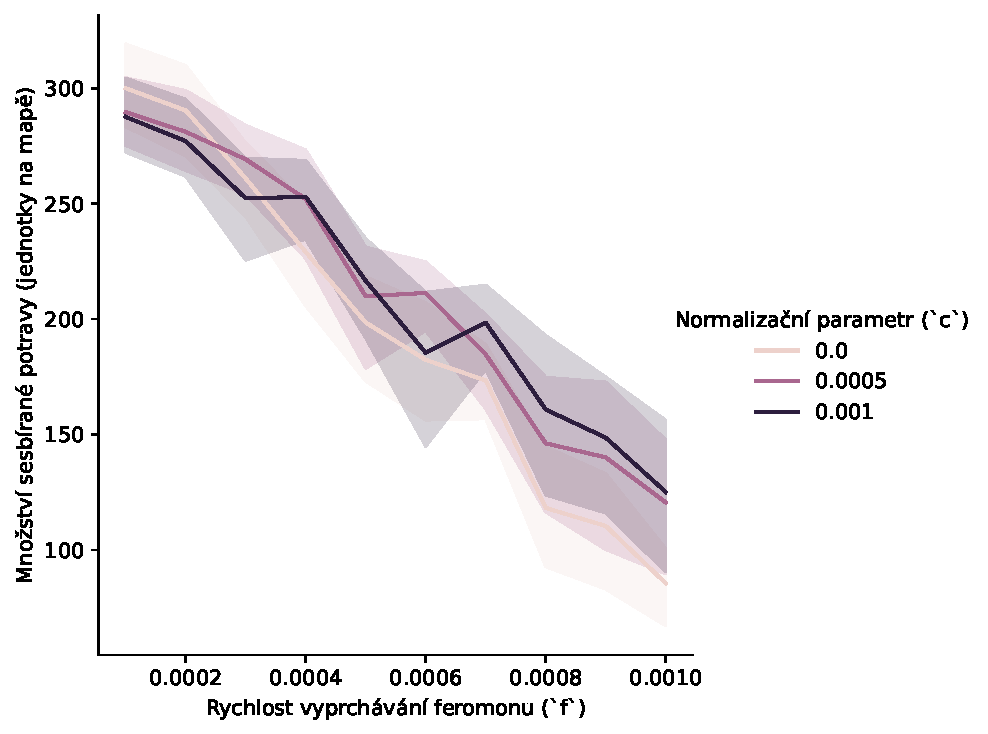
\includegraphics[width=0.9\linewidth]{images/grid_search_1_fade.pdf}
  \caption{Množství sesbírané potravy je vyšší v případě částečně náhodného
  vlivu feromonu (varianty $c=0.0005$ a $c=0.001$). Množství sesbírané 
  potravy klesá téměř lineárně s rostoucí rychlostí vyprchávání feromonu 
  (parametr $f$).}
  \label{fig:grid_search_1_fade}
\end{figure}


\begin{figure}[tb]
  \centering
  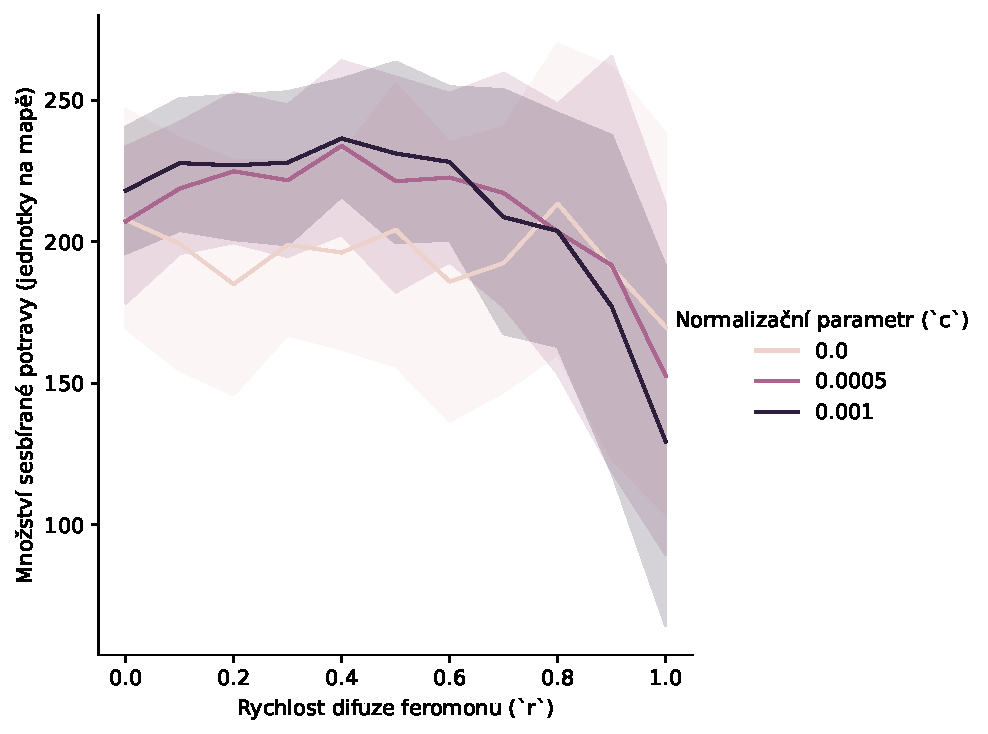
\includegraphics[width=0.9\linewidth]{images/grid_search_1_difusion.pdf}
  \caption{Množství sesbírané potravy je vyšší v případě částečně náhodného
  vlivu feromonu (varianty $c=0.0005$ a $c=0.001$). Množství sesbírané 
  potravy není téměř ovlivněno změnou rychlosti difuze (parametr $r$). 
  Výrazný pokles pozorujeme až kolem hodnoty $0.8$ a vyšší.}
  \label{fig:grid_search_1_difusion}
\end{figure}


V druhé části výběru parametru jsme se zabývali pouze volbou parametru
rychlosti vyprchávání feromonu $f \in (0.0001, 0.001)$ a rychlosti 
difuze $r \in (0, 1)$. Porovnávali jsme množství sesbírané potravy za 
$8000$ iterací simulace. S pevně zvolenými parametry jako v případě 
první části a dále s parametrem $c = 0.0005$, jehož hodnotu jsme 
odvodili v první části. Z výsledků jsme podobně jako v případě 
první části vybrali 20 variant s nejvyšším počtem nasbírané potravy
a vypočítali aritmetický průměr hodnot parametrů $f$ a $r$. Vypočtené 
hodnoty jsou následující $f = 0.00021$ $r = 0.495$. Závislost vlivu 
parametrů je srovnatelný s výsledky první části a je znázorněn
grafy (\ref{fig:grid_search_2_fade}) a (\ref{fig:grid_search_2_difusion}).


\begin{figure}[tb]
  \centering
  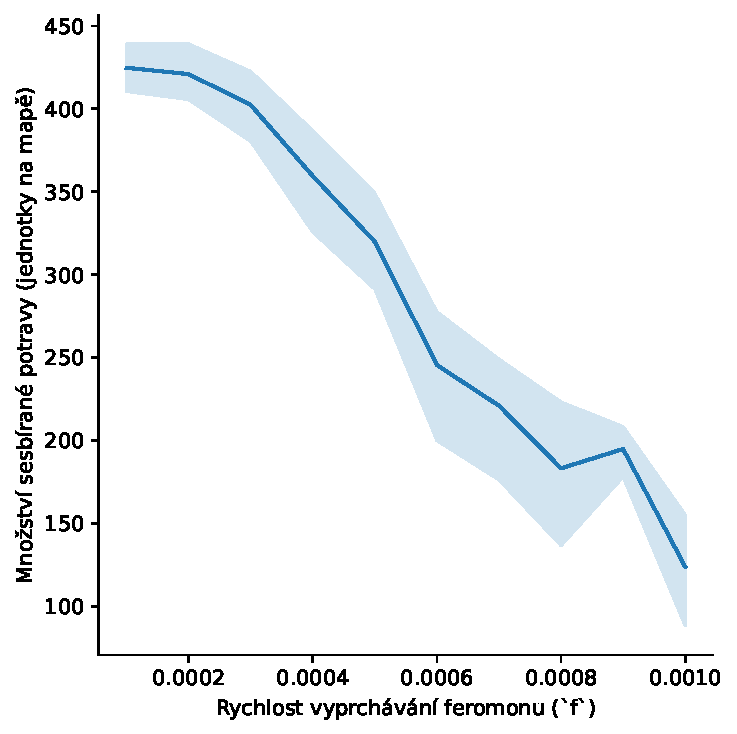
\includegraphics[width=0.9\linewidth]{images/grid_search_2_fade.pdf}
  \caption{Množství sesbírané potravy klesá téměř lineárně s rostoucí 
  rychlostí vyprchávání feromonu (parametr $f$). Vyjímkou jsou hodnoty
  parametru $f$ do $0.0002$ u nichž je rozdíl téměř zanedbatelný.}
  \label{fig:grid_search_2_fade}
\end{figure}


\begin{figure}[tb]
  \centering
  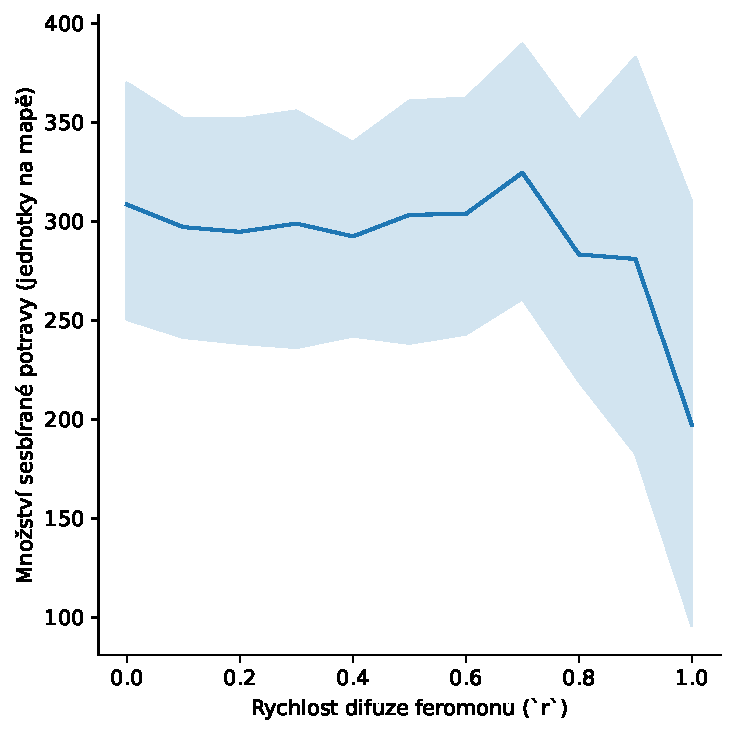
\includegraphics[width=0.9\linewidth]{images/grid_search_2_difusion.pdf}
  \caption{Množství sesbírané potravy není téměř ovlivněno změnou rychlosti 
  difuze (parametr $r$). Výrazný pokles pozorujeme až kolem hodnoty $0.8$ 
  a vyšší.}
  \label{fig:grid_search_2_difusion}
\end{figure}


\subsection*{Popis experimentů}
Hlavní část experimentů byla zaměřena na charakteristiku chování mravenců v
různých variantách prostředí s různým počtem jedinců (parametr $n$ v rozmezí 
$(0, 50)$) a různou maximální vzdáleností pro detekci hledaného objektu 
(parametr $d$ v rozmezí $(20, 2000)$). V experimentech jsme se zaměřovali 
na poměr sesbírané potravy vůči celkovému počtu potravy na mapě po uplynutí
$8000$ iterací simulace. Na základě výběru parametrů popsaných výše jsme 
pevně zvolili následující hodnoty zbylých parametrů:

\begin{itemize}
  \item $f = 0.00021$
  \item $p = 0.02$
  \item $r = 0.495$
  \item $c = 0.0005$
\end{itemize}


TODO: popsat vysledky vyberu parametru

TODO: popis nastavení modelu a vlastností modelu


% Please use pisikabst.bst. You may your own *.bib file.
\bibliographystyle{pisikabst}
\bibliography{bibfile}



\end{document}